%; whizzy chapter
% -initex iniptex -latex platex -format platex -bibtex jbibtex -fmt fmt
% 以上 whizzytex を使用する場合の設定。

%     Kansai Debian Meeting resources
%     Copyright (C) 2007 Takaya Yamashita
%     Thank you for Tokyo Debian Meeting resources

%     This program is free software; you can redistribute it and/or modify
%     it under the terms of the GNU General Public License as published by
%     the Free Software Foundation; either version 2 of the License, or
%     (at your option) any later version.

%     This program is distributed in the hope that it will be useful,
%     but WITHOUT ANY WARRANTY; without even the implied warranty of
%     MERCHANTABILITY or FITNESS FOR A PARTICULAR PURPOSE.  See the
%     GNU General Public License for more details.

%     You should have received a copy of the GNU General Public License
%     along with this program; if not, write to the Free Software
%     Foundation, Inc., 51 Franklin St, Fifth Floor, Boston, MA  02110-1301 USA

%  preview (shell-command (concat "evince " (replace-regexp-in-string "tex$" "pdf"(buffer-file-name)) "&"))
% 画像ファイルを処理するためにはebbを利用してboundingboxを作成。
%(shell-command "cd image200708; ebb *.png")

%%ここからヘッダ開始。

\documentclass[mingoth,a4paper]{jsarticle}
\usepackage{kansaimonthlyreport}
\usepackage[dvips]{xy}
\usepackage{ulem}

% 日付を定義する、毎月変わります。
\newcommand{\debmtgyear}{2013}
\newcommand{\debmtgdate}{22}
\newcommand{\debmtgmonth}{9}
\newcommand{\debmtgnumber}{76}

\begin{document}

\begin{titlepage}

% 毎月変更する部分、本文の末尾も修正することをわすれずに

 第\debmtgnumber{}回 関西 Debian 勉強会資料

\vspace{2cm}

\begin{center}
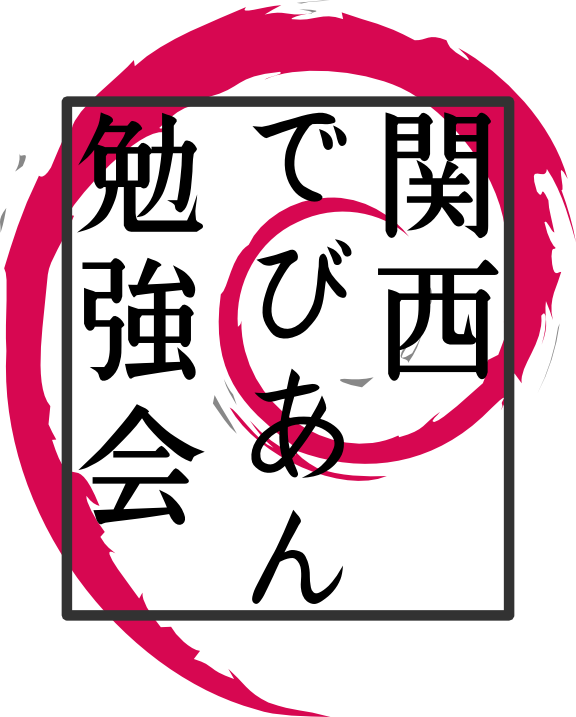
\includegraphics{image200802/kansaidebianlogo.png}
\end{center}

\begin{flushright}
\hfill{}関西 Debian 勉強会担当者 佐々木・倉敷・のがた・かわだ・八津尾 \\
\hfill{}\debmtgyear{}年\debmtgmonth{}月\debmtgdate{}日
\end{flushright}

\thispagestyle{empty}
\end{titlepage}

\dancersection{Introduction}{Debian JP}

\vspace{1em}

 関西Debian勉強会はDebian GNU/Linuxのさまざまなトピック
 (新しいパッケージ、Debian特有の機能の仕組、Debian界隈で起こった出来事、
 などなど)について話し合う会です。

 目的として次の三つを考えています。
 \begin{itemize}
  \item MLや掲示板ではなく、直接顔を合わせる事での情報交換の促進
  \item 定期的に集まれる場所
  \item 資料の作成
 \end{itemize}

 それでは、楽しい一時をお過ごしください。

\newpage

\begin{minipage}[b]{0.2\hsize}
 {\rotatebox{90}{\fontsize{80}{80}
{\gt 関西 Debian 勉強会}}}
\end{minipage}
\begin{minipage}[b]{0.8\hsize}
\hrule
\vspace{2mm}
\hrule
\setcounter{tocdepth}{1}
\tableofcontents
\vspace{2mm}
\hrule
\end{minipage}

\dancersection{最近のDebian関係のイベント報告}{Debian JP}

\subsection{第 75 回関西 Debian 勉強会}

75 回目の関西 Debian 勉強会は 8 月 25 日(日)に、福島区民センターで行な
われました。

セッションは倉敷さんによる「puppet による構成管理の実践」でした。

puppet を使い始められるきっかけとなったと思います。また、いつもとは違う
ワークショップ形式の開催はいかがだったでしょうか。アンケートに回答いた
だくなど感想をください。

\subsection{第 104 回東京エリア Debian 勉強会}
104 回目の東京エリア Debian 勉強会は 9 月 21 日(土)にあんさんぶる荻窪で
開催予定でしたが、キャンセルとなりました。来月の OSC 2013 Tokyo/Fall で
出張開催される予定です。

\subsection{Debian Project}

「Bits from the Release」
\footnote{\url{http://lists.debian.org/debian-devel-announce/2013/08/msg00006.html}}
で Jessie の開発に次の新しいアイデアが提案されています。
\begin{screen}
  \begin{itemize}
  \item Changing testing migration (NEW-TEST)
  \item Key-packages and automated removals (AUTO-RM)
  \item Automating Architecture (re-)Qualification (ARCH)
  \item Roll call for porters (ROLL-CALL)
  \end{itemize}
\end{screen}

また、「Call for Jessie Release Goals」
\footnote{\url{http://lists.debian.org/debian-devel-announce/2013/09/msg00001.html}}
で Jessie のリリースゴール提出が呼び掛けられました。リリースゴールをみ
ると次のリリースでの大きな変更点がわかりますので確認してみてください。
今のところ「pkg-php-tools」があがっています。

Debian Project News が2ヶ月ぶりに配信されました。近いうちに日本語訳も配
信されるでしょう。翻訳、査読に協力しようと思われる方は「Debian JP Documentation メーリングリスト」
\footnote{\url{http://www.debian.or.jp/community/ml/openml.html\#docML}}
を購読してください。

\dancersection{事前課題}{Debian JP}

今回の課題は以下の通りです。
\begin{screen}
  \begin{enumerate}
  \item サウンドデバイスを持つPCあるいはARMボードにDebian GNU/Linux Wheezy をインストールし、パッケージ「alsa-base」、「libasound2」、
    \sout{「libasound2-data」、}「libasound2-plugins」、「alsa-utils」をインストールしておいてください。

  \item 「dgit」を動かせる環境を用意しておいてください。

     (パッケージを持ってくるだけで wheezy 環境にもインストールできます。)

  \end{enumerate}
\end{screen}

参加者の皆さんの解答は以下の通りです:

\begin{prework}{ かわだてつたろう }
  \begin{enumerate}
  \item  sid 環境にインストールしました。
  \item インストールしましたが、clone に失敗しました。
  \end{enumerate}
\end{prework}

\begin{prework}{ 西山和広 }
  \begin{enumerate}
  \item 仮想マシンで用意しました。
  \item 1で用意した環境を使える予定です。
  \end{enumerate}
\end{prework}

\begin{prework}{ 木下 }
  \begin{enumerate}
  \item 間に合えばですが、PANDABOARDで試してみます。
  \item こちらも間に合えばやっておきます。
  \end{enumerate}
\end{prework}

\begin{prework}{ おくの }
勉強会までに間に合わせます$><$
\end{prework}

\begin{prework}{ 川江 }
了解です。
\end{prework}

\begin{prework}{ yyatsuo }
用意しておきます
\end{prework}

\begin{prework}{ 山城の国の住人 久保博 }
  \begin{enumerate}
  \item はい、インストールしました
  \item はい、ソースパッケージを wheezy 環境でビルドしてインストールしました。
  \end{enumerate}
\end{prework}

\begin{prework}{ 佐々木洋平 }
インストールしました。dgit 便利そうですね。
\end{prework}

\begin{prework}{ 坂本 貴史 }
(無回答)
\end{prework}

\begin{prework}{ 西原 }
各パッケージインストール済みPCをを持参します。
\end{prework}

\begin{prework}{ lurdan }
  \begin{enumerate}
  \item すでにインストールされていました
  \item すみません動きません
  \end{enumerate}
\end{prework}

\dancersection{Linuxとサウンドシステム}{坂本 貴史}

\subsection{ALSAの概要}
\begin{itemize}
\item Advanced Linux Sound Architecture
\item ALSAはLinuxのためのサウンドデバイスを開発するプロジェクト
\item 1998年あたりに始まる
\item LinuxディストリビューションおよびAndroidがALSAを利用してデバイスとの入出力を行う
\item 主要な開発者はLinuxディストリビューター、半導体メーカー、Androidメーカーに在籍
\end{itemize}

\subsection{音声入出力に関係するハードウェアとその制御及びデータ}
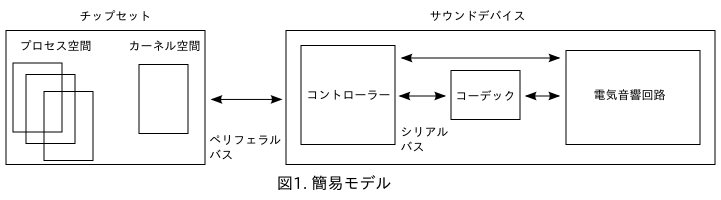
\includegraphics[width=14.0cm]{image201309/alsa.png}

\subsection{ALSAのユーザー/カーネル空間のインターフェイス}
\begin{itemize}
\item ALSAはLinux専用のサブシステム。Unixライクにデバイスノードへのファイル操作を行ってデバイスを操作する
\item サウンドデバイスはキャラクター型のデバイス。/dev/snd以下に設けられる。
\item open(2)/read(2)/write(2)/close(2)だけでデバイスを制御するのは難しい。
\item ioctl(2)で柔軟な操作を行う。libasound2で専用APIを提供。
\item procfsの/proc/asound以下のノードでALSAの基本情報を提供している
\end{itemize}

\subsection{Linuxカーネル/ドライバーとALSA}
\subsubsection{デバイスクラスとALSA}
\begin{itemize}
\item Linuxにはデバイスクラスがある。soundcoreモジュールがsoundクラスを提供する。ALSAはsoundクラスのドライバー。
\item ALSA Coreは各ドライバーに対し、以下の機能を提供
  \begin{itemize}
  \item ユーザー空間とのインターフェイスを提供するAPI
  \item Linuxのdriver/base(sysfs含む)に対する共通API
  \item Linuxのprocfsに対する共通API
  \item Open Sound Systemとの互換レイヤ
  \item その他ヘルパー関数
  \end{itemize}
\item ALSAのドライバーは、Linuxの各バスドライバーが提供するAPIを利用し、ALSAのインターフェイスとデバイスを中継する役割を果たす
\end{itemize}

\subsection{ALSAのカーネルランドコンフィグレーション}
\begin{itemize}
\item ALSAのカーネルランドはLinuxのローダブルモジュールとして実装されている
\item modprobeを使い、ローダブルモジュールにオプションを渡すことができる
\end{itemize}

\subsection{ALSAのユーザーランドコンフィグレーション}

\begin{itemize}
\item libasound2は設定ファイルのパース機能を持つ
\item libasound2はシステムレベル、ユーザーレベルでランタイム設定を変更できる
\item libasound2はプラグイン構造を持つ
\end{itemize}

\subsection{ALSAのアプリケーション}
\begin{itemize}
\item alsa-utils、PulseAudio、Jack Audio Connection Kit
\end{itemize}

\subsection{圧縮データとgstreamer/libav}
\begin{itemize}
\item サウンドシステムは基本、PCMデータを扱うよう作られている
\item 圧縮データからPCM標本を取り出す処理をどこかで入れる必要がある
\end{itemize}

\subsection{Androidとtinyalsa、AudioFlinger}
\begin{itemize}
\item AndroidはカーネルランドにLinuxカーネルを使っていて、ALSAを利用している
\item ユーザーランドはlibasound2ではないtinyalsaを使う
\end{itemize}

\subsection{その他の話題}
\begin{itemize}
\item salsa、COMPRESS/tinycompress、Audio Visual Bridge (AVB)、FirewireとALSA
\end{itemize}


\dancersection{dgit でソースパッケージを触ってみる}{倉敷 悟}

\dancersection{今後の予定}{Debian JP}

\subsection{関西 Debian 勉強会}

次回、第 77 回関西 Debian 勉強会は 10 月 27 日(日)に港区民センターで開催予定です。

11 月は 11 月 8 日(金)、9 日(土)と大阪南港 ATC ITM 棟で開催される KOF2013 に出張予定です。


\subsection{東京エリア Debian 勉強会}

第 104 回東京エリア Debian 勉強会はは 10 月 19 日(土)、20 日(日)に行なわれる OSC 2013 Tokyo/Fall での出張開催予定です。

%
% 冊子にするために、4の倍数にする必要がある。
% そのための調整
\dancersection{メモ}{}
\mbox{}\newpage
 %% \mbox{}\newpage
 %% \mbox{}\newpage

\printindex
%\cleartooddpage

 \begin{minipage}[b]{0.2\hsize}
  \rotatebox{90}{\fontsize{80}{80} {\gt 関西 Debian 勉強会} }
 \end{minipage}
 \begin{minipage}[b]{0.8\hsize}

 \vspace*{15cm}
 \rule{\hsize}{1mm}
 \vspace{2mm}
 
\includegraphics[width=2cm]{image200502/openlogo-nd.eps}
 \noindent \Large \bf Debian 勉強会資料\\ \\
 \noindent \normalfont \debmtgyear{}年\debmtgmonth{}月\debmtgdate{}日 \hspace{5mm}  初版第1刷発行\\
 \noindent \normalfont 関西 Debian 勉強会 (編集・印刷・発行)\\
 \rule{\hsize}{1mm}
 \end{minipage}

\end{document}
